\documentclass{exam}
\usepackage{graphicx} 


%Format Header and footer
\pagestyle{headandfoot}
\header{\footnotesize Klass:\\Namn:}{\Large\textbf{Systematik}}{\footnotesize  BIOBIO01 - 2024\\Viktor Arohlén}
\headrule
\footrule
\setlength{\columnsep}{0.25cm}
%\setlength{\columnseprule}{1pt}
\footer{}{Sida \thepage}{}
%\extrafootheight{-2cm}

\begin{document}
\vspace{5mm} %5mm vertical space
\begin{center}
\fbox{\fbox{\parbox{6in}{\centering
\textbf{Kortsvarsfrågor}: svara kortfattat (E-C)
}}}
\end{center}
\vspace{5mm} %5mm vertical space
\begin{questions}
\question Rangordna följande begrepp \textit{hierarkiskt}

\begin{itemize}
  \item Ordning 
  \item Släkte
  \item Domän
  \item Art
  \item Stam
  \item Rike
\end{itemize}
\vspace{5mm} %5mm vertical space
\question
Homo georgicus, Homo antecessor samt Ardipithecus ramidus beskrivs som tre olika människoarter/förmänniskor. Vilka två av dessa tror du är närmast släkt? \textit{Motivera ditt} svar!
\vspace{30mm} 
\question
Vilka tre huvudsakliga domäner delar vi in allt liv i? Vad skiljer domänerna åt?
\vspace{30mm} 
\question
Svampar, djur och växter tillhör en av dessa domäner.
\begin{parts}
\part Vilken?
\part Vad kallas grupperingsnivån med svampar, djur och växter?
\part Vad kännetecknar de tre olika grupperna?
\end{parts}
\break
\question 
Vilka är närmast släkt? \textit{Motivera!}
\begin{itemize}
  \item Tall
  \item Björnmossa
  \item Tulpan
\end{itemize}
\vspace{30mm}
\question
Vilka av följande djurgrupper är äldst, evolutionärt sett? \textit{Motivera!}
\begin{itemize}
  \item Plattmaskar
  \item Aborre
  \item Gråvarg
\end{itemize}
\vspace{5mm}
\break
\begin{center}
\fbox{\fbox{\parbox{6in}{\centering
\textbf{Frisvarsfrågor}: svara mer utförligt (E-A)}}}
\end{center}
\begin{figure}[h]
    \centering
    \includegraphics[width=0.5\linewidth]{Carl_von_Linné_webb.jpg}
\end{figure}
\vspace{5mm} %5mm vertical space
\question Carl Von Linné bestämde arternas släktskap med ett \textit{morfologiskt perspektiv}. 
\begin{parts}
\part Vad innebär ett \textit{morfologiskt perspektiv}?
\part Vad finns det för nackdelar med perspektivet?
\end{parts}
\vspace{60mm}
\question \textit{Prokaryoter} och \textit{protister} är exempel på gamla grupperingar inom systematiken. 
\begin{parts}
\part Vilka grupper av arter ingår i dem?
\part Varför vill vi undvika att använda dem idag?
\end{parts}

\break
\vspace{5mm}
\question "Maskar" är en \textbf{parafyletisk grupp} bestående av stammarna rundmaskar, plattmaskar och ringmaskar.
\begin{parts}
\part Varför är det en parafyletisk grupp?
\part Vilka stammar hade behövt ingå för att den ska vara monofyletisk?
\end{parts}
\vspace{100mm}
\question Däggdjuren delas upp i tre grupper.
\begin{parts}
\part Vilka är grupperna och vad skiljer dem åt?
\part Vilken av dem är evolutionärt äldst? Motivera!
\end{parts}
\break
\vspace{5mm} %5mm vertical space
\question På nästa sida finns ett fylogenetiskt släktträd för \textbf{SARS-CoV-2 viruset} som orsakade covid-19-pandemin. Utöver SARS-CoV-2 hittar vi SARS-Cov som orskade SARS-epidimin i Asien under 2003. Vi hittar också MERS-CoV som skapade oro för ytterligare en epidemi i Saudiarabien 2012. Dessa är alla röd-markerade.

I samma släktträd hittar vi också ett antal vanliga förkylningsvirus (HCov HKU1, HCoV OC43, HCoV 229E och HCoVNL63). Dessa är grönmarkerade.

Övriga virus är närbesläktade virus som inte smittar människan utan andra arter.
\vspace{5mm} 
\begin{parts}
\part Vilka av de rödmarkerade virusen är \textit{närmast släkt}?
\vspace{5mm} 
\part Vilket virus är SARS-CoV-2 \textit{närmsta föregångare}? Motivera!
\vspace{5mm} 
\part Ibland får man höra att förkylning och covid orsakas av liknande virus. Utifrån släktträdet, hur sant är det påståendet? Motivera!
\vspace{5mm} 
\part De rödmarkerade virusen har alla uppkommit genom \textit{zoonos}. Det vill säga att virus muterat och smittar \textit{mellan} arter. Utifrån släktträdet och informationen, ser du någon risk för att liknande virus skulle kunna uppkomma i framtiden? Motivera!
\end{parts}
\begin{figure}
    \centering
    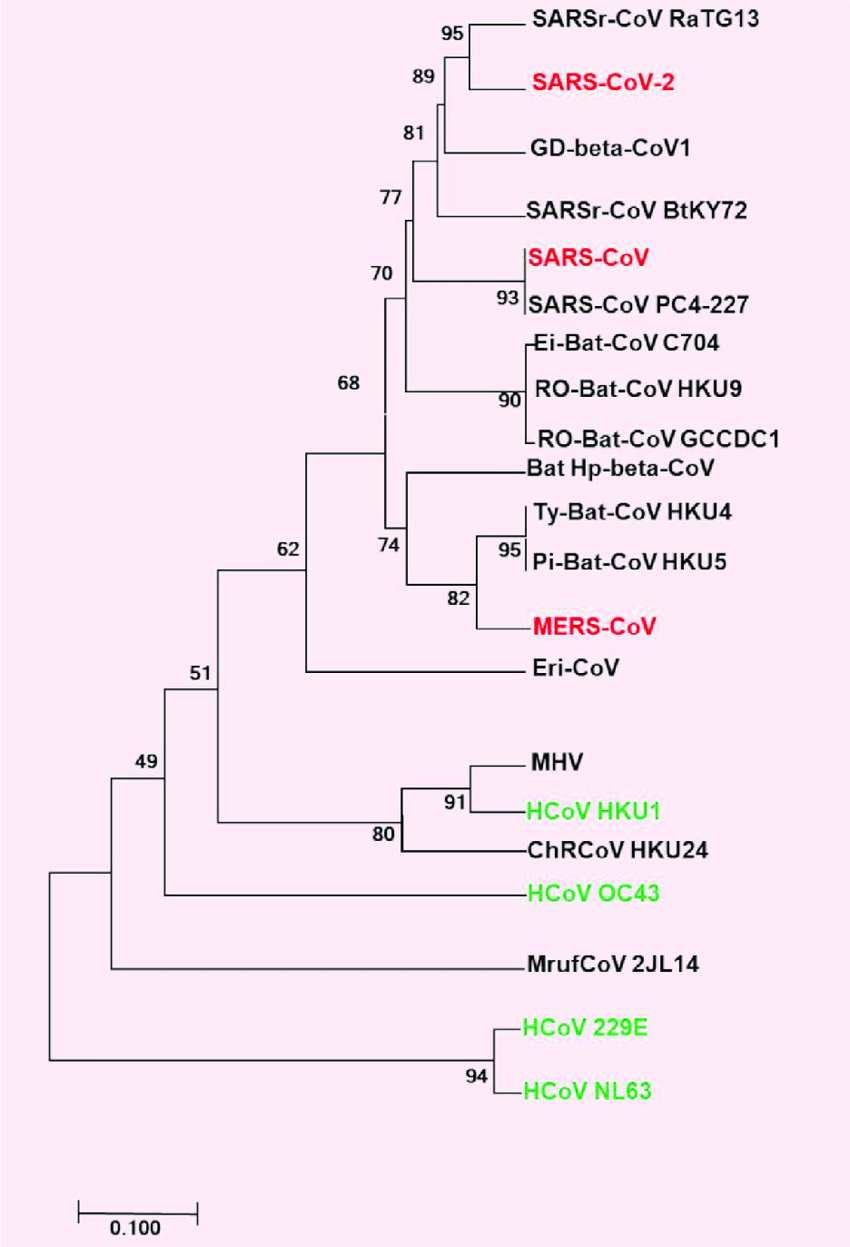
\includegraphics[width=1\linewidth]{Phylogenetic-tree-of-representative-species-of-SARS-CoV-2-SARS-CoV-and-MERS-CoV-Red.png}
\end{figure}
\end{questions}





\end{document}
